\documentclass{beamer}

\usepackage{graphicx}
\usetheme{metropolis}
\usepackage[latin1]{inputenc}
\usepackage{tikz}
\usetikzlibrary{shapes,arrows}

\metroset{progressbar=frametitle}
\metroset{background=dark}

\setbeamercolor{palette primary}{bg=black, fg=white}
\setbeamercolor{background canvas}{parent=palette primary}
\setbeamercolor{normal text}{fg=white}
\setbeamercolor{progress bar}{use=palette primary, fg=red}

\makeatletter
\setlength{\metropolis@progressinheadfoot@linewidth}{4pt}
\setlength{\metropolis@titleseparator@linewidth}{4pt}
\makeatother

\title[BB84]{BB84}
\subtitle{A Quantum Key Distribution Protocol}
\author[Team 37]{Lakshika, Shreya}
\date{July 2020}

\begin{document}

\begin{frame}
	\titlepage
\end{frame}

\begin{frame}
	\frametitle{Overview}
	 Simulation of BB84 Protocol
\end{frame}


\begin{frame}[standout]
    \begin{columns}
        \column{0.35\linewidth}
            \centering
            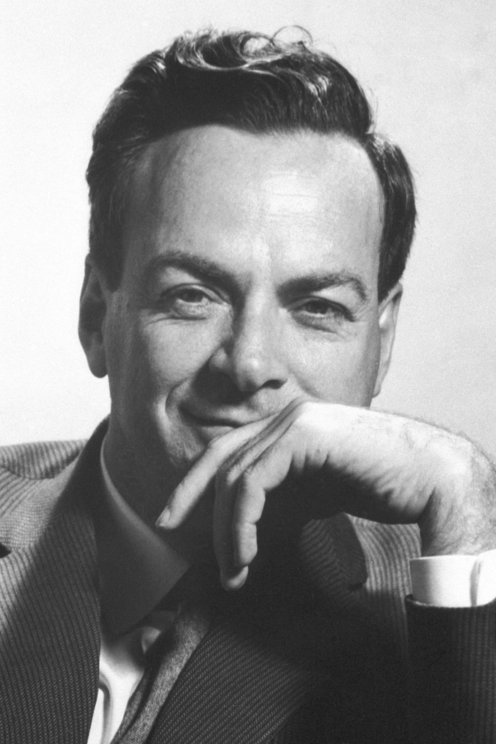
\includegraphics{feynman.jpg}
        \column{0.58\linewidth}
            \emph{Nature isn’t classical, dammit, and if you want to make a simulation of nature, you’d better make it quantum mechanical...}
        \begin{flushright}
            - Richard Feynman
        \end{flushright}
    \end{columns}
\end{frame}


\begin{frame}{Technology Stack}
	\begin{itemize}
		\item Qiskit - An SDK for Quantum Computing
		\item IBM Q - IBM Quantum Experience to access IBM's quantum computers via the cloud
        \item Python Libraries
	\end{itemize}
\end{frame}


\begin{frame}{Quantum Key Distribution}
    \begin{itemize}[<+->]
        \item Key distribution is an important step in Cryptographic protocols
        \item Current protocols assume computational limitations
        \item \begin{itemize}
                \item Quantum Cryptography
                \item Post-Quantum Cryptography
              \end{itemize}
        \item The first QKD protocol by Bennet and Brassard in 1984
     \end{itemize}
\end{frame}


\begin{frame}{The Quantum World}
     \begin{columns}
         \column{0.45\linewidth}
                \centering
                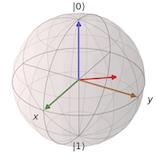
\includegraphics{qubit.png}
        \column{0.73\linewidth}
            \begin{itemize}[<+->]
                \item \textbf{Qubit} - Basic unit of Quantum Information
                \item Bases and Measurement
                \item Communication channels
                      \begin{itemize}
                            \item A one-way physical Quantum channel
                            \item An authenticated two-way classical ideal channel
                      \end{itemize}
                \end{itemize}
    \end{columns}
\end{frame}


\begin{frame}{Protocol - Quantum Phase}
    \begin{itemize}[<+->]
        \item Generation of a random bitstring and bases 
		\item Quantum transmission of encoded bits
		\item Measurement by the receiver
		\item Public comparison of bases and sifting
	\end{itemize}
\end{frame}


\begin{frame}{Protocol - Information Reconciliation}
	The process of cleaning the keys from errors
	\begin{itemize}[<+->]
		\item Error estimation
		\item Low Density Parity Check codes based reconciliation
	\end{itemize}
\end{frame}


\begin{frame}{Protocol - Privacy Amplification}
	\begin{itemize}[<+->]
	    \item Distillation of a highly secret key from a partially secure string by public discussion
		\item Shrinks the possible exposed information over the communication channels to almost zero
		\item 2-Universal hash functions are used
	\end{itemize}
\end{frame}


\begin{frame}{The Protocol at a glance !}
% Define block styles
    \tikzstyle{decision} = [diamond, draw]
    %text width=7em, text badly centered, node distance=3cm, inner sep=0pt]i
    \tikzstyle{block} = [rectangle, draw, fill=red]
    %text width=10em, text centered, rounded corners, minimum height=2em]
    \tikzstyle{block2} = [rectangle, draw, rounded corners, node distance=6cm]
    \tikzstyle{block3} = [rectangle, draw, rounded corners, node distance=1.5cm]
\tikzstyle{line} = [draw, -latex']
    \tikzstyle{cloud} = [draw, ellipse, node distance=7cm, text width=11em]
    %minimum height=1em]
    \tikzstyle{cloud1} = [draw, ellipse, node distance=1.5cm]
    
\begin{tikzpicture}[node distance = 1.5cm, auto]
    % Place nodes
    \node [block] (QT) {Quantum Transmission};
    \node [block, below of=QT] (PC) {Public Comparison};
    \node [block, below of=PC] (CPE) {Channel parameter estimation};
    \node [block3, below of=CPE] (QBER) {QBER to validate secret};
    \node [block, below of=QBER] (R) {Information Reconciliation};
    \node [block, below of=R] (A) {Privacy Amplification};
    \node [block2, right of=QT] (keys) {Alice's key, Bob's key};
    \node [block2, right of=PC] (sift) {Sifted keys of Alice and Bob};
    \node [block2, right of=QBER] (exit) {Exit protocol \\ (QBER > Threshold)};

    \path [line] (QT) -- (PC);
    \path [line] (QT) -- (keys);
    \path [line] (PC) -- (CPE);
    \path [line] (PC) -- (sift);
    \path [line] (CPE) -- (QBER);
    \path [line] (QBER) -- (exit);
    \path [line] (QBER) -- (R);
    \path [line] (R) -- (A);
\end{tikzpicture}
\end{frame}


\begin{frame}{References}
    \begin{tabular}{r l}
        \footnotesize{\textbf{The Protocol}} & \footnotesize{Lecture Notes by \emph{Univerity of Berkeley}} \\
            \footnotesize{\textbf{LDPC codes}} & \footnotesize{\emph{Alan Mink and Anastase Nakassis}}, \footnotesize{"Practical Strategies} \\
             & \footnotesize{for QKD Key Production"} \\
            \footnotesize{\textbf{Standard Matrices}} & \footnotesize{\emph{P.Venkateshwari and M.Anbuselvi}, "Decoding performance} \\ 
             & \footnotesize{of binary and non-binary LDPC codes"} \\
             & \footnotesize{\emph{Mario Milicevic et al.}, "Key Reconciliation with LDPC} \\ 
              & \footnotesize{Codes for Long-Distance Quantum Cryptography"} \\
            \footnotesize{\textbf{Privacy Amplification}} & \footnotesize{\emph{H. F. Chau et al.}, "Practical issues in quantum} \\ 
              & \footnotesize{key-distribution post-processing"} \\
            \footnotesize{\textbf{Eavesdropping}} & \footnotesize{\emph{John Smolin et al.}, "Experimental Quantum Cryptography"} \\
    \end{tabular}
\end{frame}
    

\begin{frame}{Difficulties faced}
	\begin{itemize}
		\item Getting started with Quantum Computing
        \item In choosing a sub-domain
        \item Unsure about the language and tools to use
		\item Figuring out Information Reconciliation part
	\end{itemize}
\end{frame}


\begin{frame}{Learnings}
	\begin{itemize}
		\item Explored the domain of Quantum Computing
		\item Learnt the basics of Quantum Cryptography
		\item Collecting, reading research papers and trying to understand them
		\item Got introduced to Coding theory
	\end{itemize}
\end{frame}


\end{document}
